\input ../SlidePreamble
\input ../preamble
\newcommand{\float}{\mathrm{Float}}

\begin{document}

{\Huge
  \centerline{\bf TTIC 31230,  Fundamentals of Deep Learning}
  \vfill
  \centerline{David McAllester, Autumn   2024}
  \vfill
  \centerline{\bf Maximizing Mutual Information}
  \vfill
  \centerline{\bf Contrastive Coding}
  \vfill
  \centerline{\bf Cotraining}
  \vfill
  \centerline{\bf The Visual Transformer (ViT)}
  \vfill
  \vfill


\slide{Maximizing Mutual Information}

Assume a population of pairs $(x,y)$.

 \vfill
\begin{itemize}
\item $x$ might be an image and $y$ might be the text of a caption for image $x$ (CLIP).

\vfill
\item $x$ might be an video frame and $y$ video frame a second later.

\vfill
\item $x$ might be a window of a sound wave and $y$ a later window (Wav2Vec).

\vfill
\item $x$ and $y$ are different transformations of an image $z$ such as translation, rotation, color shift, or cropping. (SimCLR,DINO)
\end{itemize}

\slide{Maximizing Mutual Information}

{\bf The Information Bottleneck Method} Tishby, Pereira, Bialek, (1999).


\vfill
Assume a distribution on pairs $(x,y)$ and an encoder $P_\enc(z|x)$.

\vfill
$$\enc^* = \argmax_\enc I(z,y) - \beta I(z,x)$$

\slide{Maximizing Mutual Information}

The methods discussed here --- contrastive coding and cotraining --- can be interpreted as optimizing only the first term in the
information bottleneck.

\vfill
We take the encoder to be deterministic $\enc(x) \in R^d$ and maximize mutual information with $y$.

$$\enc^* = \argmax_\enc\; I(\enc(x),y)$$

\vfill
Here there is no incentive in this objective for $\enc(x)$ to retain information unrelated to $y$.

\slide{Maximizing Mutual Information.}

$$\enc^* = \argmax_\enc\; I(\enc(x),y)$$

\vfill
{\huge
It would be natural to try to maximize a variational lower bound on $I(\enc(x),y)$.

\vfill
In the applications discussed here we expect hundreds of bits of mutual information.

\vfill
Unfortunately one can prove that no formal lower bound
establishing hundreds of bits of mutual information  is possible without an exponential ($2^{100}$) number of training examples.

\vfill
{\bf Formal Limitations on the Measurement of Mutual Information},
David McAllester, Karl Stratos, (November 2018)
}

\slide{Surrogate Objectives and Hardness Parameters}

Since variation optimization of mutual information is not possible, contrastive learning and cotraining each introduce a surrogate objective.

\vfill
Each surrogate objective has a parameter --- the hardness parameter --- that controls the difficulty of the optimization problem.

\vfill
Increasing the hardness parameter makes training more difficult but should increase the resulting mutual information $I(\enc(x),y)$
when training is successful.

\slide{Contrastive Coding}

{\bf Representation Learning with Contrastive Predictive Coding}, van den Oord, Li and Vinyals (DeepMind, 2018)

\vfill
CLIP: {\bf Learning Transferable Visual Models From Natural Language Supervision} (OpenAI, February 2021)

\slide{The Contrastive Coding Desiderata}

We draw a batch of pairs $(x_1,y_1),\ldots,(x_B,y_B)$.

\vfill
We select one of the $x$ values.

\vfill
We train a classifier that, when given one of the $x$ values and the batch $(y_1,\ldots,y_B)$ of $y$ values, must determine which $y$ was paired with the given $x$.


\slide{The Contrastive Coding Surrogate Objective}

We train two encoders $\enc_x$ and $\enc_y$ with $\enc_x(x) \in R^d$ and $\enc_y(y) \in R^d$.

{\huge
$$\enc_x^*,\enc_y^* = \argmin_{\enc_x,\enc_y}\; \begin{array}{cl} E_{(b,x_b,y_1,\ldots,y_B)}\;&\left[-\ln P_{\enc_x,\enc_y}(b|x_b,y_1,\ldots,y_B)\right] \\
+  E_{(b,y_b,x_1,\ldots,x_B)}&\left[-\ln P_{\enc_x,\enc_y}(b|y_b,x_1,\ldots,x_B)\right]\end{array}$$

\vfill
\begin{eqnarray*}
P_{\enc_x,\enc_y}(b|x,y_1,\ldots,y_B) & = & \softmax_b\; \enc_x(x)^\top\enc_y(y_b) \\
P_{\enc_x,\enc_y}(b|y,x_1,\ldots,x_B) & = & \softmax_b\; \enc_y(y)^\top\enc_x(x_b) \\
\end{eqnarray*}
}

\slide{The Contrastive Coding Hardness Parameter}


{\huge
\begin{eqnarray*}
{\cal L}(\enc_x,\enc_y) & = & E_{(b,x_b,y_1,\ldots,y_B)}\left[-\ln P_{\enc_x,\enc_y}(b|x_b,y_1,\ldots,y_B)\right] \\
& \;\;\;+ & E_{(b,y_b,x_1,\ldots,x_B)}\left[-\ln P_{\enc_x,\enc_y}(b|y_b,x_1,\ldots,x_B)\right]
\end{eqnarray*}

\vfill
The hardness parameter is the batch size $B$.  Making $B$ large makes the classification task harder.

\vfill
In CLIP $B$ = $2^{15}$ = 32,768.

\slide{Zero-Shot Image Classification}

\centerline{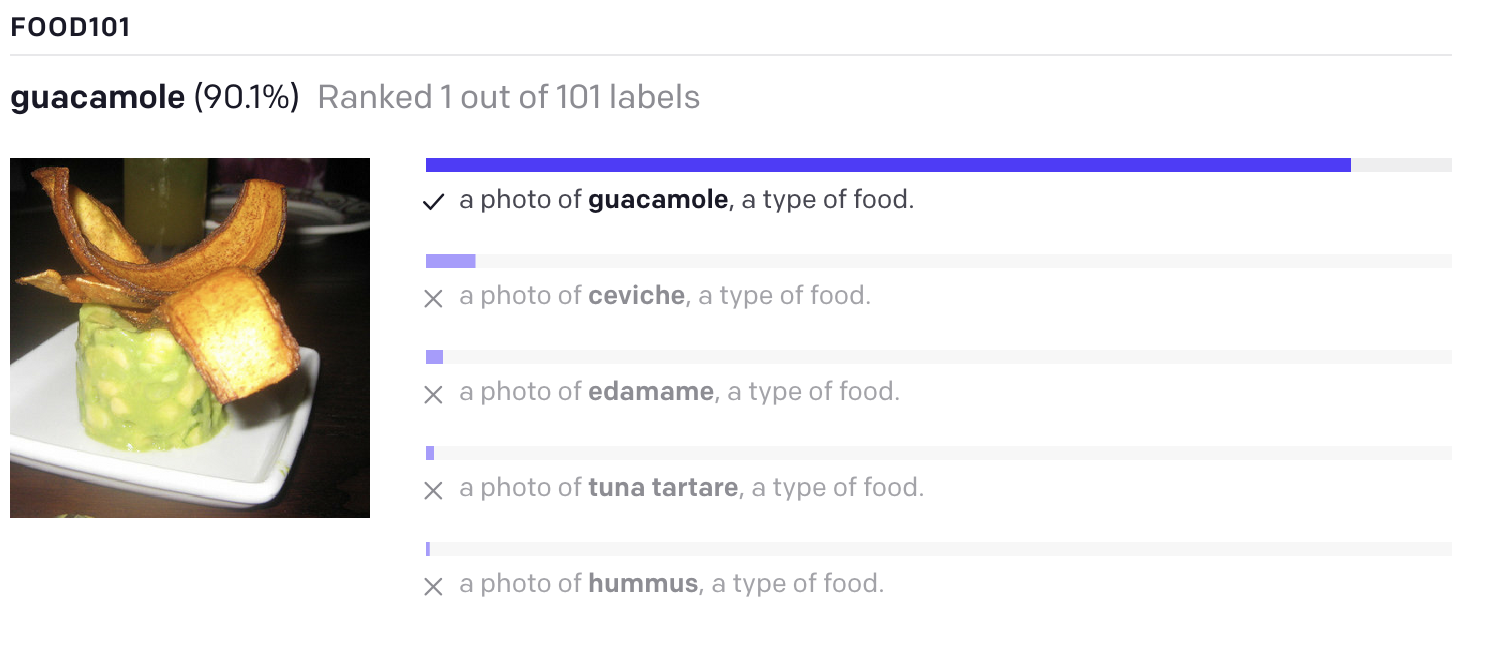
\includegraphics[width = 7in]{\images/CLIP0}}

\slide{Zero-Shot Image Classification}

\centerline{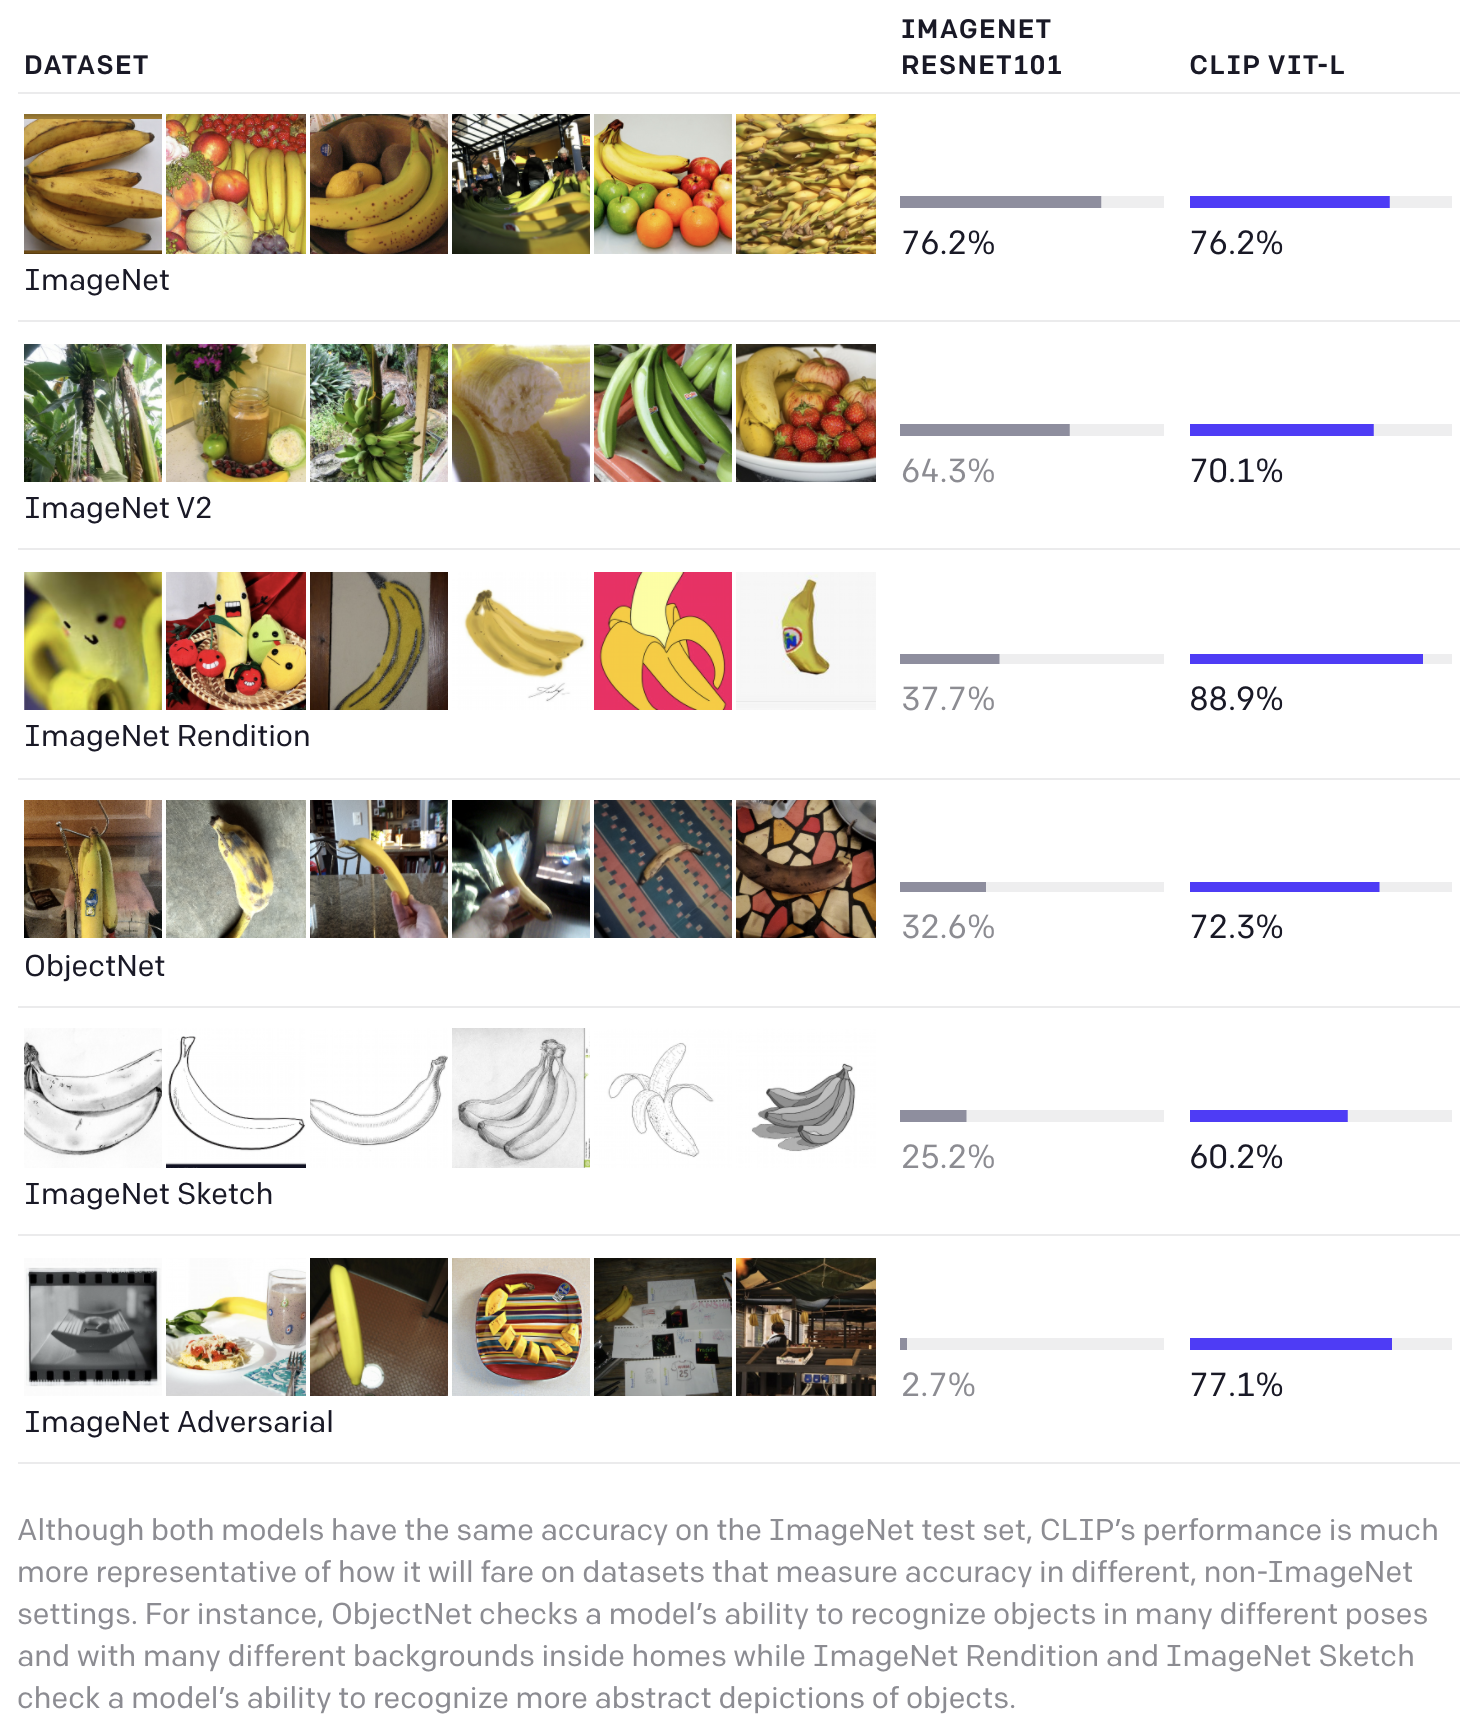
\includegraphics[height= 5in]{\images/CLIP1}}


\slide{Cotraining}

{\bf Combining labeled and unlabeled data with co-training} Avrim Blum, and Tom Mitchell (1998)

\vfill
{\bf PAC Generalization Bounds for Co-training}, Dasgupta, Littman, McAllester (2001)

\vfill
DINOv1: {\bf Emerging Properties in Self-Supervised Vision Transformers}, (Meta, Inria, April 2021)

\vfill
iBOT: {\bf Image BERT Pre-Training with Online Tokenizer},
Zhou et al. (ByteDance, January 2022)

\vfill
DINOv2: {\bf Learning Robust Visual Features without Supervision}, (Meta, Inria, February 2024)

\slide{Cotraining}

We again consider a population distribution on pairs $(x,y)$.

\vfill
In cotraining we assume a label set $k \in \{1,\ldots,K\}$.

\vfill
The labels have no a-priori meaning.  Meaning will emerge from the training.

\vfill
We train two classifiers $P_\Phi(k|x)$ and $P_\Psi(k|y)$ under a cotraining objective.

\slide{Cotraining Desiderata}

{\huge
In cotraining we seek to find two classifiers $P_\Phi(k|x)$ and $P_\Psi(k|y)$ such that on typical pairs $(x,y)$ the two classifiers agree on the label.

\begin{itemize}
\item[(1)] For a given pair $(x,y)$ we want each classifier to be confident in its label.  Formally, we want that in expectation over the draw of a pair $(x,y)$ the entropies
$H(P_\Phi(k|x))$ and $H(P_\Psi(k|y))$ are both small.

\item[(2)] For a given pair $(x,y)$ we want the classifiers to agree on the label. Formally, we want that in expectation over a draw of a pair $(x,y)$ the cross-entropies
$H(P_\Phi(k|x),P_\psi(k|y))$ and $H(P_\psi(k|y),P_\Phi(k|x))$ are both small.

\item[(3)] We want that over different draws of $(x,y)$ the distributions of predicted labels covers all the labels.  Formally, we want the marginal distributions $P_\Phi(k)$
and $P_\Psi(k)$ to have large entropy.
\end{itemize}
}


\slide{The Cotraining Surrogate Objective}

$$\Phi^*,\Psi^* = \argmin_{\Phi,\Psi}\;E_{(x,y)\sim \pop} \left\{\begin{array}{cl}&H(P_\Phi(k|x),P_\Psi(k|y)) \\ +& H(P_\Psi(k|y),P_\Phi(k|x)) \\ \\ - & \beta(H(P_\Phi(k)) + H(P_\Psi(k)))\end{array}\right.$$

\vfill
Here we have subsumed the criterion (1) -- that the classifiers are confident -- into the cross-entropy terms.  Making the cross entropies small requires confidence of both classifiers as well as agreement.

\slide{The Cotraining Hardness Parameter}

$$\Phi^*,\Psi^* = \argmin_{\Phi,\Psi}\;E_{(x,y)\sim \pop} \left\{\begin{array}{cl}&H(P_\Phi(k|x),P_\Psi(k|y)) \\ +& H(P_\Psi(k|y),P_\Phi(k|x)) \\ \\ - & \beta(H(P_\Phi(k)) + H(P_\Psi(k)))\end{array}\right.$$

\vfill
The Hardness parameter is $K$, the number of labels.  Getting agreement on all labels, when all labels are used, is hard when the number of labels is large.

\vfill
in DINOv2 $K$ = $2^{10} + 2^9$ = 1536.

\slide{Collapse of the Surrogate Objective}

$$\Phi^*,\Psi^* = \argmin_{\Phi,\Psi}\;E_{(x,y)\sim \pop} \left\{\begin{array}{cl}&H(P_\Phi(k|x),P_\Psi(k|y)) \\ +& H(P_\Psi(k|y),P_\Phi(k|x)) \\ \\ - & \beta(H(P_\Phi(k)) + H(P_\Psi(k)))\end{array}\right.$$

\vfill
SGD on the this surrogate objective collapses into making both $P_\Phi(k|x)$ and $P_\Psi(k|y)$ uniform in $k$.

\vfill
This maximizes $H(P_\Phi(k))$ and $H(P_\Psi(k))$ and gives

$$\Phi = \argmin_\Phi E_{(x,y)}\;H(P_\Phi(k|x),P_\Psi(k|y)) + H(P_\Psi(k|y),P_\Phi(k|x))$$
$$\Psi = \argmin_\Psi E_{(x,y)}\;H(P_\Phi(k|x),P_\Psi(k|y)) + H(P_\Psi(k|y),P_\Phi(k|x))$$

\vfill
Hence this is a local optimum of SGD.

\slide{Collapse of the Surrogate Objective}

More generally whenever $P_\Phi(k|x)$ and $P_\Psi(k|y)$ agree we have.

$$\Phi = \argmin_\Phi E_{(x,y)}\;H(P_\Phi(k|x),P_\Psi(k|y)) + H(P_\Psi(k|y),P_\Phi(k|x))$$
$$\Psi = \argmin_\Psi E_{(x,y)}\;H(P_\Phi(k|x),P_\Psi(k|y)) + H(P_\Psi(k|y),P_\Phi(k|x))$$

\vfill
So the gradients on $\Phi$ and $\Psi$ vanish.

\vfill
We can improve the cross-entropies by reducing both $H(P_\Phi(k|x))$ and $H(P_\Psi(k|y))$ simultaneously.
However, the amount of improvement is quadratic (second order) in the change in parameters.

\vfill
It seems that SGD is attracted to saddle points!

\slide{DINOv1}

We will discuss the simpler version DINOv1. DINOv2 is similar but with a variety of engineering improvements.

\vfill
The main contribution of DINO is a method for avoiding collapse of the training into uniform distributions $P_\Phi(k|x)$ and $P_\Psi(k|y)$.

\vfill
They their innovation ``self-distillation''.

\vfill
The basic idea of self-distillation is to do a brute-force enforcement the desiderata (1)-(3) given above.

\slide{Self-Distillation}

They construct a ``teacher network'' $\tilde{P}_\Phi(k|x)$ which uses the same parameters as $P_\Phi(k|x)$ but which is modified to enforce
(encourage) the desiderata.

\vfill
They then replace the cross-entropy losses in the cotraining objective with

$$H(sg(\tilde{P}_\Phi(k|x)),P_\Psi(k|y))\;\mbox{and}\;H(sg(\tilde{P}_\Psi(k|y)),P_\Phi(k|x)).$$

\vfill
We train $P_\Psi(k|y)$ to model $\tilde{P}_\Phi(k|x)$
and train $P_\Phi(k|x)$ to model $\tilde{P}_\Psi(k|y)$. sg is the stop-gradient operator.

\slide{Why the stop-gradient sg?}

$$H(\tilde{P}_\Phi(k|x),P_\Psi(k|y)) = E_{k \sim \tilde{P}_\Phi(k|x)}\left[-\ln P_\Psi(k|y)\right]$$

\vfill
Computing the gradient with respect to $\Phi$ is problematic in any case --- optimizing a sampling distribution is problematic in general.

\vfill
We simply avoid the issue by not trying to compute this gradient.

\vfill
We sample from $\tilde{P}_\Phi(k|x)$ and compute gradients on $\Psi$.

\slide{Encouraging the Desiderata}

\vfill
{\bf Increasing Confidence (Sharpening):} They put a temperature parameter into the softmax of $\tilde{P}_\Phi(k|x)$.
This allows $\tilde{P}_\Psi(k|x)$ to be defined at a lower temperature (higher $\beta$) which ``sharpens'' the distribution.

\vfill
{\bf Diversifying the Label Usage (Centering):} For each category $k$ we compute an EMA over the draw of pairs $(x,y)$ of the
score (the logit) $s_\Phi(k,x)$.  Denote this EMA value by $\overline{s}(k)$.  The softmax defining the distribution $\tilde{P}_\Phi(k|x)$ is then

$$\tilde{P}_\Phi(k|x) = \softmax_k\;\beta(s_\Phi(k|x) - \overline{s}(k))$$

\slide{DIVOv1 PyTorch Pseudo-code}

\centerline{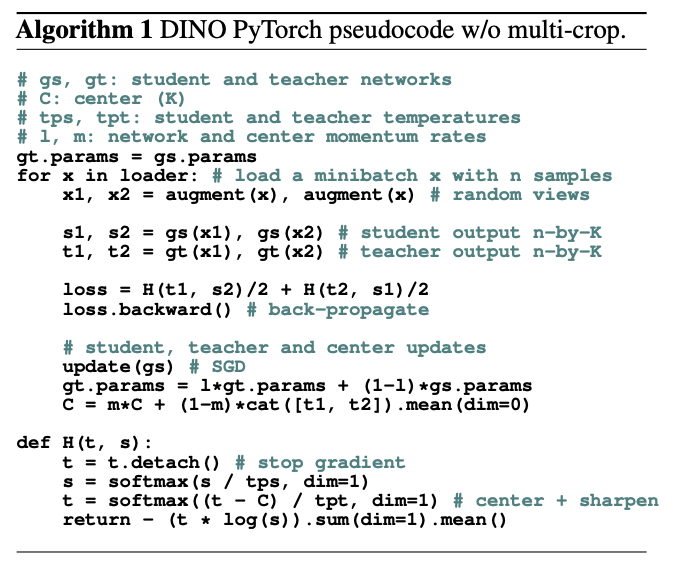
\includegraphics[height= 5in]{\images/DINO1}}

\slide{Results for DINOv2}

\centerline{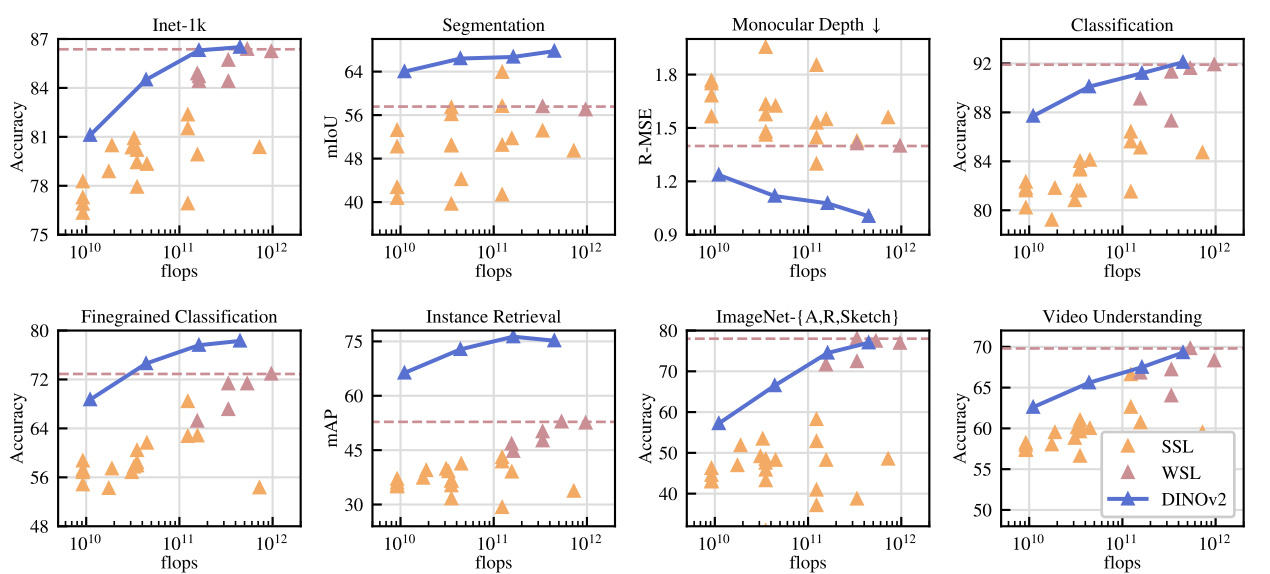
\includegraphics[width= 7in]{\images/DINO4}}

\slide{The Vision Transformer (ViT)}

Part of the motivation for DINOv1 (Meta, April 2021) was to demonstrate the power of visual transformers (Google Brain, October 2020).

\vfill
{\bf An Image is Worth 16x16 Words: Transformers for Image Recognition at Scale}, Alexey Dosovitskiy et al. (Oct 2020, Google Brain)

\slide{ViT}

An image $I$ with height $X$, width $Y$ and $C = 3$ color channels has shape
$I[X,Y,C]$.  In a ViT this is processed by a linear layer with stride $s$ resulting in a layer $L$ with shape $L[X/s,Y/s,N]$.
This processing is equivalent to a Conv2d layer with stride $s$ but
without an activation function (there is no ReLU).

$$\mbox{for}\;x,y,n,\Delta x, \Delta y, c\;\;\;L[x,y,n] \;\pluseq\; W[n,\Delta x,\Delta y,c]I[sx+\Delta x,sy+\Delta Y,c]$$

\vfill
In the original ViT paper the stride $s$ is taken to be 16 (hence the title). DINOv2 uses $s$ = 14.

\vfill
Presumably for each neuron $n$ the tensor $W[n,\Delta X,\Delta Y,C]$ converges on some Haar wavelet.

\slide{ViT}

We now have a tensor $L(X,Y,N)$. We treat this as $X \times Y$ positions with an ``embedding vector'' at each position.

\vfill
At each position the embedding vector is concatenated with a position embedding. The position embeddings can be trained so there is no need
to make a distinction between ``linear'' vs. ``spatial'' position embeddings (this would presumably not be true for relative position embeddings.)

\vfill
An additoinal non-image  position is added to represent the image as a whole. The vector computed for the additonal position, which I will write as $\enc_x(x)$, is interpreted as the feature vector
for image $x$.

\vfill
In DINOv2 each component $\enc_x(x)[k]$ of the image embedding is interpreted as the score of label $k$.

\slide{Attention Gives Segmentation in DINOv1}

\centerline{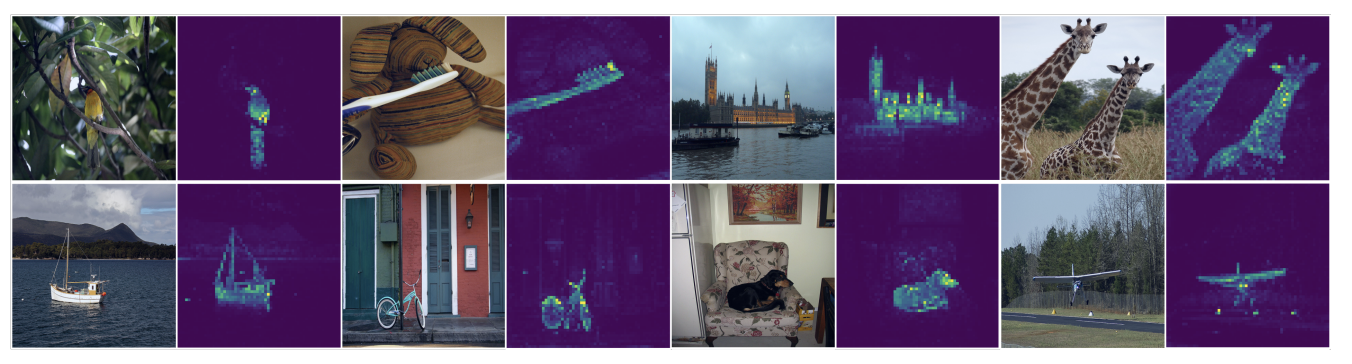
\includegraphics[width = 8.5in]{\images/DINO2}}

\vfill
This is showing the attention that the whole image position pays to the other image positions.

\slide{PCA Gives Part Matching in DINOv2}

\centerline{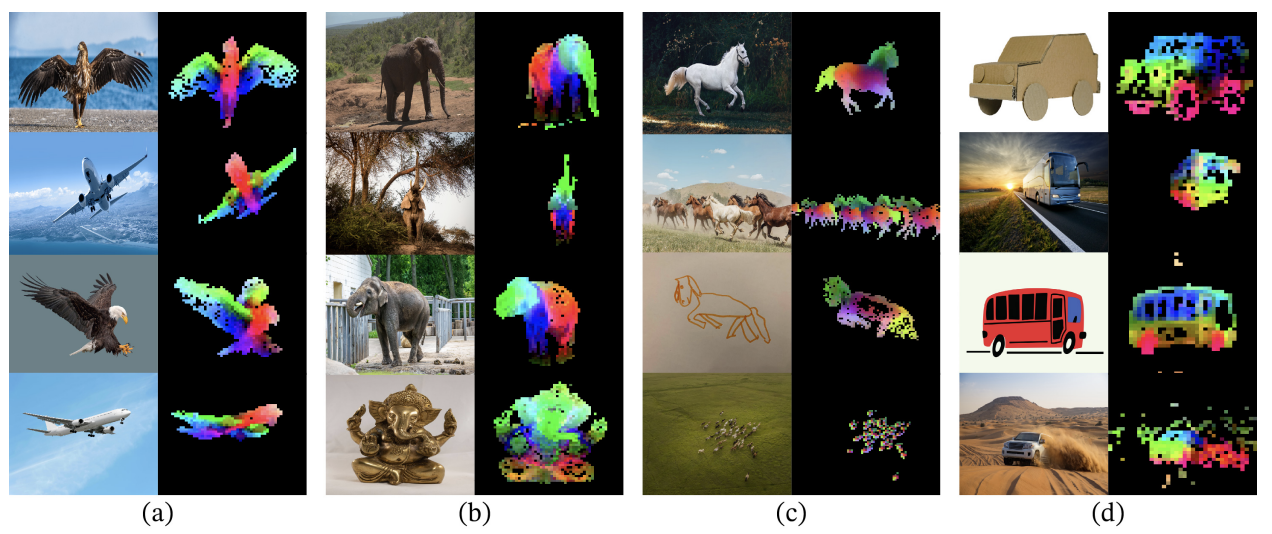
\includegraphics[width = 6in]{\images/DINO3}}

\vfill
For each column we pool the top transformer layer vectors across the four images of the column and do PCA on that pool of vectors.

\vfill
Each image is segmented by thresholding the largest PCA component.

\vfill
The three colors in the image then correspond to the strength of the three largest PCA components. We then get part matching across different images.

\slide{END}

}
\end{document}

